\cmfnewsection{Criação de Componentes e Bibliotecas}{./logos/fundo_tese}{0.15}







%%%%%%%%%%%%%%%%%%%%%%%%%%%%%%%%%%%%%%%%%%%%%%%%
%%%%%%%%%%%%%%%%%%%%%%%%%%%%%%%%%%%%%%%%%%%%%%%%
%%%%%%%%%%%%%%%%%%%%%%%%%%%%%%%%%%%%%%%%%%%%%%%%
%%%%%%%%%%%%%%%%%%%%%%%%%%%%%%%%%%%%%%%%%%%%%%%%
\begin{frame}{Encapsulando Circuitos: {\it Component Wizard}}
\centering


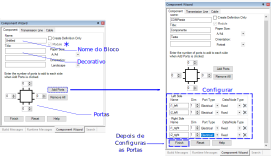
\includegraphics[width=0.75\linewidth]{./figuras/Componentes/wizard}


\end{frame}





%%%%%%%%%%%%%%%%%%%%%%%%%%%%%%%%%%%%%%%%%%%%%%%%
%%%%%%%%%%%%%%%%%%%%%%%%%%%%%%%%%%%%%%%%%%%%%%%%
%%%%%%%%%%%%%%%%%%%%%%%%%%%%%%%%%%%%%%%%%%%%%%%%
%%%%%%%%%%%%%%%%%%%%%%%%%%%%%%%%%%%%%%%%%%%%%%%%
\begin{frame}{Encapsulando Circuitos: Resultado}
\centering


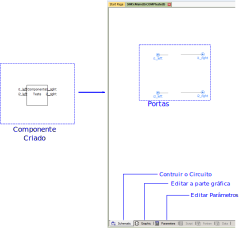
\includegraphics[width=0.45\linewidth]{./figuras/Componentes/componenteTeste}


\end{frame}




%%%%%%%%%%%%%%%%%%%%%%%%%%%%%%%%%%%%%%%%%%%%%%%%
%%%%%%%%%%%%%%%%%%%%%%%%%%%%%%%%%%%%%%%%%%%%%%%%
%%%%%%%%%%%%%%%%%%%%%%%%%%%%%%%%%%%%%%%%%%%%%%%%
%%%%%%%%%%%%%%%%%%%%%%%%%%%%%%%%%%%%%%%%%%%%%%%%
\begin{frame}{Encapsulando Circuitos: Montando o Esquemático}
\centering


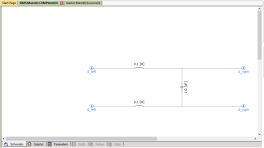
\includegraphics[width=0.75\linewidth]{./figuras/Componentes/schematico}


\end{frame}







%%%%%%%%%%%%%%%%%%%%%%%%%%%%%%%%%%%%%%%%%%%%%%%%
%%%%%%%%%%%%%%%%%%%%%%%%%%%%%%%%%%%%%%%%%%%%%%%%
%%%%%%%%%%%%%%%%%%%%%%%%%%%%%%%%%%%%%%%%%%%%%%%%
%%%%%%%%%%%%%%%%%%%%%%%%%%%%%%%%%%%%%%%%%%%%%%%%
\begin{frame}{Encapsulando Circuitos: Testando}
\centering


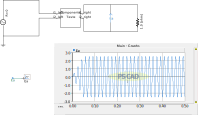
\includegraphics[width=0.75\linewidth]{./figuras/Componentes/Testando}


\end{frame}






%%%%%%%%%%%%%%%%%%%%%%%%%%%%%%%%%%%%%%%%%%%%%%%%
%%%%%%%%%%%%%%%%%%%%%%%%%%%%%%%%%%%%%%%%%%%%%%%%
%%%%%%%%%%%%%%%%%%%%%%%%%%%%%%%%%%%%%%%%%%%%%%%%
%%%%%%%%%%%%%%%%%%%%%%%%%%%%%%%%%%%%%%%%%%%%%%%%
\begin{frame}{Encapsulando Circuitos: {\it Decorando o Bloco}}
\centering


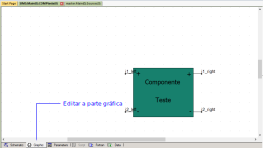
\includegraphics[width=0.75\linewidth]{./figuras/Componentes/grafica}


\end{frame}






%%%%%%%%%%%%%%%%%%%%%%%%%%%%%%%%%%%%%%%%%%%%%%%%
%%%%%%%%%%%%%%%%%%%%%%%%%%%%%%%%%%%%%%%%%%%%%%%%
%%%%%%%%%%%%%%%%%%%%%%%%%%%%%%%%%%%%%%%%%%%%%%%%
%%%%%%%%%%%%%%%%%%%%%%%%%%%%%%%%%%%%%%%%%%%%%%%%
\begin{frame}{Encapsulando Circuitos: Testando, de novo}
\centering


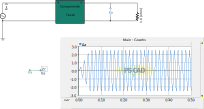
\includegraphics[width=0.75\linewidth]{./figuras/Componentes/Testando2}


\end{frame}




%%%%%%%%%%%%%%%%%%%%%%%%%%%%%%%%%%%%%%%%%%%%%%%%
%%%%%%%%%%%%%%%%%%%%%%%%%%%%%%%%%%%%%%%%%%%%%%%%
%%%%%%%%%%%%%%%%%%%%%%%%%%%%%%%%%%%%%%%%%%%%%%%%
%%%%%%%%%%%%%%%%%%%%%%%%%%%%%%%%%%%%%%%%%%%%%%%%
\begin{frame}{Programando componentes com FORTRAN}
\centering

\begin{columns}


\column{0.5\linewidth}
\begin{itemize}
\item Criar um bloco seguindo os passos anteriores
\vspace*{1cm}
\item Demarcar a opção {\it Module}
\vspace*{1cm}
\item Programar o bloco na aba script
\end{itemize}

\column{0.5\linewidth}
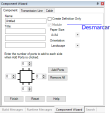
\includegraphics[width=0.75\linewidth]{./figuras/Componentes/componenteFortran}

\end{columns}




\end{frame}




%%%%%%%%%%%%%%%%%%%%%%%%%%%%%%%%%%%%%%%%%%%%%%%%
%%%%%%%%%%%%%%%%%%%%%%%%%%%%%%%%%%%%%%%%%%%%%%%%
%%%%%%%%%%%%%%%%%%%%%%%%%%%%%%%%%%%%%%%%%%%%%%%%
%%%%%%%%%%%%%%%%%%%%%%%%%%%%%%%%%%%%%%%%%%%%%%%%
\begin{frame}{Programando componentes com FORTRAN: Componente A}
\centering

Componente que soma uma constante $K$ a todos os elementos de um vetor. Ou seja:
\vspace*{0.5cm}

\begin{equation*}
\mathbf{y}[n] = \mathbf{x}[n] + K 
\end{equation*}
\vspace*{0.5cm}

$\mathbf{y}$ - Vetor com $N$ posições (saída do bloco)
\vspace*{0.5cm}

$\mathbf{x}$ - Vetor com $N$ posições (entrada do bloco)
\vspace*{0.5cm}

$K$ - Constante


\end{frame}





%%%%%%%%%%%%%%%%%%%%%%%%%%%%%%%%%%%%%%%%%%%%%%%%
%%%%%%%%%%%%%%%%%%%%%%%%%%%%%%%%%%%%%%%%%%%%%%%%
%%%%%%%%%%%%%%%%%%%%%%%%%%%%%%%%%%%%%%%%%%%%%%%%
%%%%%%%%%%%%%%%%%%%%%%%%%%%%%%%%%%%%%%%%%%%%%%%%
\begin{frame}{Programando componentes com FORTRAN: Componente A}
\centering

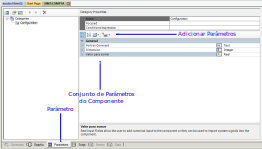
\includegraphics[width=0.75\linewidth]{./figuras/Componentes/FortranA_parameter}

\end{frame}




%%%%%%%%%%%%%%%%%%%%%%%%%%%%%%%%%%%%%%%%%%%%%%%%
%%%%%%%%%%%%%%%%%%%%%%%%%%%%%%%%%%%%%%%%%%%%%%%%
%%%%%%%%%%%%%%%%%%%%%%%%%%%%%%%%%%%%%%%%%%%%%%%%
%%%%%%%%%%%%%%%%%%%%%%%%%%%%%%%%%%%%%%%%%%%%%%%%
\begin{frame}{Programando componentes com FORTRAN: Componente A}
\centering

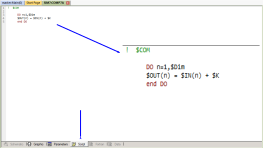
\includegraphics[width=0.75\linewidth]{./figuras/Componentes/FortranA_script}

\end{frame}




%%%%%%%%%%%%%%%%%%%%%%%%%%%%%%%%%%%%%%%%%%%%%%%%
%%%%%%%%%%%%%%%%%%%%%%%%%%%%%%%%%%%%%%%%%%%%%%%%
%%%%%%%%%%%%%%%%%%%%%%%%%%%%%%%%%%%%%%%%%%%%%%%%
%%%%%%%%%%%%%%%%%%%%%%%%%%%%%%%%%%%%%%%%%%%%%%%%
\begin{frame}{Programando componentes com FORTRAN: Componente B}
\centering

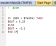
\includegraphics[width=0.45\linewidth]{./figuras/Componentes/FortranB_script}

\end{frame}





%%%%%%%%%%%%%%%%%%%%%%%%%%%%%%%%%%%%%%%%%%%%%%%%
%%%%%%%%%%%%%%%%%%%%%%%%%%%%%%%%%%%%%%%%%%%%%%%%
%%%%%%%%%%%%%%%%%%%%%%%%%%%%%%%%%%%%%%%%%%%%%%%%
%%%%%%%%%%%%%%%%%%%%%%%%%%%%%%%%%%%%%%%%%%%%%%%%
\begin{frame}{Guardando componentes em uma Biblioteca}
\centering

\begin{columns}


\column{0.5\linewidth}

\begin{itemize}
\item Crie uma biblioteca
\vspace*{1cm}
\item No workspace, Copie a definição do componente do seu projeto
\vspace*{1cm}
\item Cole na seção de definições da biblioteca
\end{itemize}
\vspace*{1cm}

\column{0.5\linewidth}
\centering
\vspace*{1cm}

\includegraphics[width=0.75\linewidth]{./figuras/Componentes/lib}


\end{columns}

\end{frame}